\documentclass[aspectratio=169,10pt]{beamer}
\mode<presentation>
{
  %%\usetheme{Copenhagen}
  \usetheme{Warsaw}
  %%\setbeamercovered{transparent}
}

\setcounter{tocdepth}{1}
\AtBeginSection[]
{
  \begin{frame}<beamer>
    \frametitle{Contenido de la charla}
    \tableofcontents[currentsection,currentsubsection]
  \end{frame}
}
\usepackage[utf8]{inputenc}
\usepackage{times}
\usepackage[T1]{fontenc}
\usepackage[scanall]{psfrag}
\usepackage{bibunits}
\usepackage[spanish]{babel} 
\usepackage{listings}
\usepackage{xcolor}
\usepackage{pgf,pgffor} 
\usepackage{tikz}
\usetikzlibrary{arrows}

\lstdefinestyle{base}{  breaklines=true,
                    basicstyle=\footnotesize,
                    numbers=none,
                    numberstyle=\tiny, numbersep=5pt,
                    breaklines=true,
                    tabsize=2, captionpos=b , stepnumber=1,aboveskip=0pt, belowskip=0pt,
                    moredelim=**[is][\color{red}]{@}{@},
                    moredelim=**[is][\color{blue}]{@2}{@},
                    moredelim=**[is][\only<4->{\color{green}}]{@4}{@},
                    moredelim=**[is][\only<5->{\color{blue}}]{@5}{@},
        }

\title{Aplanado eficiente de grandes modelos Modelica}
\author[M.Botta] {Mariano Botta } 
\institute[UNR] % (optional, but mostly needed)
{ FCEIA, UNR }
\date {Agosto 2015}

\subject{Talks}
\begin{document}

\begin{frame}
  \titlepage
\end{frame}

 
\section{Motivaciones y Objetivos}  

\begin{frame}{Motivaciones}
    \begin{itemize}
     \item Modelado, Simulación y Control en Tiempo Real con Aplicaciones en Electrónica de Potencia.
     \item Trabajar con sistemas a grandes escalas.
     \item Simulación en paralelo utilizando los métodos de cuantificación de estado.       
     \item Aprovechar las ventajas de Modelica para describir modelos grandes.
    \end{itemize}
\end{frame}

\begin{frame}{Objetivos}
    \begin{itemize}
     \item Mantener las caracteristicas de Modelica en las sucesivas etapas de compilación.
     \item Especificamente, en la etapa de Aplanado.
     \item Mantener definiciones de arreglos y ecuaciones \textit{for} en:
        \begin{enumerate}
            \item Reducción de clases.
            \item Resolución de conexiones.
        \end{enumerate}
    \end{itemize}
\end{frame}

\section{Conceptos Previos}

\begin{frame}{Modelica} 
    \begin{itemize}
        \item Lenguaje de modelado orientado a objetos.
        \item Modelado de sistemas complejos, con componentes mecánicos, eléctricos, electrónicos, hidráulicos, térmicos, etc.     
        \item Desarrollado por la asociación sin fines de lucro ``Modelica Asociation''.        
        \item Los modelo son descriptos en texto plano.        
        \item Entornos de desarrollo: OpenModelica, MathModelica, Dymola, etc.
        \item Librería con componentes ya definidos.
    \end{itemize}
\end{frame}
 

\begin{frame}[fragile]
\frametitle{Clases} 
\begin{columns}  
\column{.5\textwidth}  
\begin{block}{}
\begin{itemize}
    \item Define un objeto.
    \item Son instanciadas mediante la definición de variables.
    \item Tienen tres secciones:
        \begin{enumerate}
            \item Definiciones.
            \item Ecuaciones.
            \item Sentencias.
        \end{enumerate}
    \item Clases especializadas:  \textit{model}, \textit{record}, \textit{block}, \textit{connector}, \textit{function}, \textit{package}   
\end{itemize}
\end{block}{}
\column{.5\textwidth}
\begin{lstlisting}[style=base]
    class X
        // Definiciones de 
                variables y clases   
    equation
        // Ecuaciones
    statements
        // Sentencias
    end X;   
\end{lstlisting}
\end{columns}
\end{frame}

%\begin{frame}[fragile]
%\frametitle{Prefijos de Clases} 
%Prefijos de clase: \textit{model}, \textit{record}, \textit{block}, \textit{connector}, \textit{function}, \textit{package}
%\begin{itemize}
%    \item Mejoran la lectura del código:
%    \item Agregan restricciones a la clase
%\end{itemize}   
%
%\begin{columns}  
%\column{.5\textwidth}  
%\begin{lstlisting}[style=base]
%    class Circuits
%        cclass Pin
%            Real v;
%            flow Real i;
%        end Pin;
%        class Componente
%            Pin n,p;
%        equation 
%            n.v = p.v;
%        end Componente; 
%    end Circuits;   
%\end{lstlisting}
%\par
%\column{.5\textwidth}
%\begin{lstlisting}[style=base]
%    @package@ Circuits
%        @connector@ Pin
%            Real v;
%            flow Real i;
%        end Pin;
%        @model@ Componente
%            Pin n,p;
%        equation 
%            n.v = p.v;
%        end Componente; 
%    end Circuits;   
%\end{lstlisting}
%\par
%\end{columns}
%\end{frame}





\begin{frame}[fragile]
\frametitle{Herencias de Clases} 
\begin{columns}  
\column[t]{8cm}  

\begin{block}{}
\begin{itemize}
    \item Agrega significado semántico al modelo.
    \item Facilita la reutilización de código.
    \item Se utiliza la palabra reservada: \textit{extends}.
\end{itemize} 
\end{block}

\begin{block}{}
La clase hijo obtiene las caracteristicas del padre.
\end{block}

\column[t]{5cm}  
\begin{lstlisting}[style=base]
model OnePort
    Pin p;
    Pin n;
    Real v;
    Real i;
equation
    v = p.v - n.v;
    i = p.i;
    i = -n.i;
end OnePort;
model Capacitor
    @extends@ OnePort;
    parameter Real C = 1;
equation
    C * der(v) = i;
end Capacitor;
\end{lstlisting}
\end{columns}
\end{frame}

\begin{frame}[fragile]
\frametitle{Tipos de Variables} 
\begin{columns}  
\column[t]{9cm}
    \begin{itemize}
        \item \textbf{Tipos básicos}: \textit{Real}, \textit{Integer}, \textit{Boolean} y \textit{String}
        \item Las clases definen un nuevo tipo.
        \item \textbf{Sinónimos de tipos}: \\ 
              type Nombre = [Prefijos] Tipo-Existente [Array] [Modificaciones]
        \item \textbf{Prefijos de Tipo}: \textit{flow}, \textit{constant}, \textit{parameter}, \textit{discrete}, \textit{input} y \textit{output}.
    \end{itemize} 

\column[t]{5cm}
\begin{lstlisting}[style=base]
package Circuits
    type Current = flow Real;
    type Voltage = Real;
    connector Pin
        Voltage v;
        Current i;
    end Pin;
    type TenPin = Pin[10];
end Circuits;
\end{lstlisting}
\par
\end{columns}
\end{frame}

\begin{frame}[fragile]
\frametitle{Definiciones de variables} 
\begin{enumerate}
\item \textbf{Prefijos de tipos}: \textit{flow}, \textit{constant}, \textit{parameter}, \textit{discrete}, \textit{input} y \textit{output}.
\item \textbf{Tipo}: Nombre del tipo de la variable. Puede ser un tipo básico, una clase o un sinónimo de tipo.  Ejemplo: \textit{Real}, \textit{String}, \textit{Pin}, \textit{TenPin}.
\item \textbf{Nombre de la variable}. 
\item \textbf{Dimensión}: Modelica permite la definición de arreglos.
\item \textbf{Modificaciones}.
\end{enumerate}
\begin{lstlisting}[style=base]
    type TenPin = Pin[10];  
    
    TenPin pines;
    Pin pines2 [10];
\end{lstlisting}
\par

\end{frame}

\begin{frame}[fragile]
\frametitle{Modificaciones} 

\begin{columns}  
\column[T]{7cm}
\begin{block}{Aparecen en}
\begin{enumerate}
    \item Declaraciones de variables.
    \item Sinónimo de tipo.
    \item Definiciones de herencia.
\end{enumerate} 
\end{block}

\begin{block}{Podemos}
\begin{enumerate}
    \item Cambiar el valor inicial de una variable.    
    \item Redefinir una variable.
    \item Cambiar la definición de un tipo.
    \item Anidar modificaciones.
\end{enumerate}
\end{block}
\column[T]{7cm}
\begin{lstlisting}[style=base]
package Circuits
    model CircuitX
        Capacitor cap;
        Resistor res;
        ...
    equation 
    
    ...
        
    end CircuitX;
    model MainCircuit
        Capacitor x(C = 2);
        CircuitX co1 (cap(C = 10));
        CircuitX co2 (cap(C = 15));
    end MainCircuit;
end Circuits;
\end{lstlisting}

 
\end{columns}
\end{frame}

\begin{frame}[fragile,t]
\frametitle{Ecuaciones} 
\begin{block}{}
Las ecuaciones no representan una asignación, sino igualdades.\\ Pueden tener expresiones complejas de ambos lados de la igualdad y expresan una relación entre las variables.
\end{block}
\vspace{0.1cm}
\begin{columns}  
\column[t]{4cm}
Ecuaciones de Igualdad
\vspace{0.2cm}
\begin{lstlisting}[style=base]

p.v - n.v = v;
i = p.i;
i = -n.i;
\end{lstlisting} 
\column[t]{5cm}
Ecuación \textit{for}
\vspace{0.2cm}
\begin{lstlisting}[style=base]
for i in 1:N loop
    v[i] = p[i].v - n[i].v;
    i[i] = p[i].i;
    i[i] = -n[i].i;
    C[i] * der(v[i]) = i;
end for;
\end{lstlisting} 
\column[t]{4cm} 
N = 4
\vspace{0.2cm}
\begin{lstlisting}[style=base]
v[1] = p[1].v - n[1].v;       
v[2] = p[2].v - n[2].v;
v[3] = p[3].v - n[3].v;
v[4] = p[4].v - n[4].v;
\end{lstlisting} 
\end{columns}
\end{frame}

\begin{frame}[fragile]
\frametitle{Ecuaciones \textit{connect}} 
\begin{block}{Conectores}
\begin{itemize}
\item Son clases con ciertas restricciones.
\item Se definen con el prefijo \textit{connector}.
\item No tienen ecuaciones.
\item Tienen variables de dos tipos:
    \begin{itemize}
        \item Variables de potencial. Ejemplo: presión, voltaje, etc. 
        \item Variables de flujo: definidas con el prefijo flow. Ejemplo: corriente, caudal, etc.
    \end{itemize} 
\end{itemize}
\end{block}
\begin{block}{Ejemplo}
Clase Pin:
\begin{itemize}
    \item Voltaje: Variables de potencial.
    \item Corriente: Variables de flujo.
\end{itemize}
\end{block}
\end{frame}

\begin{frame}[fragile]
\frametitle{Ecuaciones \textit{connect}} 
\begin{block}{Ecuaciones \textit{connect}}
    \begin{itemize}
        \item Conectan dos clases del mismo tipo.
        \item Genera relaciones entre las variables internas de los conectores:
            \begin{itemize}
                \item Las variables de potencial dentro de una misma conexión deben ser iguales entre sí.
                \item Las variables de flujo siguen las reglas de Kirchhoff: la suma de los flujos es igual a cero. 
        \end{itemize}
    \end{itemize}
\end{block}{}

\begin{columns}  
\column[T]{8cm}
 \begin{lstlisting}[style=base,,basicstyle=\scriptsize]
    model LC_circuit
        Capacitor cap(v(start = 1));
        inductor ind(L = 2);
        ground gr;
    equation
        connect(ind.p,cap.p);
        @connect(ind.n,cap.n);@
        @connect(cap.n,gr.p);@
    end LC_circuit;
\end{lstlisting}
\column[T]{6cm}
 \begin{lstlisting}[style=base]
    // Variables de Potencial 
    ind.n.v  = cap.n.v;
    cap.n.v = gr.p.v;
    
    // Variables de flujo 
    ind.n.i + cap.n.i + gr.p.i = 0;
\end{lstlisting}
% Mencionar que se tiene que resolver a nivel global las conexiones
\end{columns}
\end{frame}


\begin{frame}[fragile]
\frametitle{Tama\~nos de un modelo} 
\begin{block}{Tamaño de la descripción}
Consideramos la cantidad de clases, variables, ecuaciones, etc. usadas.
\end{block}
\vspace{1cm}
\begin{block}{Tamaño del sistema}
Consideramos la dimensionalidad del modelo. \\
Cantidad total de variables. 
\end{block}
\end{frame}

%% antes mencionar que trabajamos con modelos con arreglos y ecuaciones for
%% Cambiar grafico por Parsing -> Flattering -> Index Reduction -> 
%% Se hace muy grande el modelo si expandimos
\begin{frame}[fragile]
\frametitle{Simulación de Modelos Modelica} 
    \begin{figure}
      \centering
      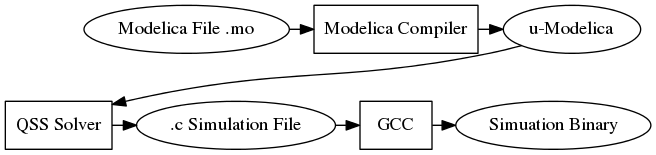
\includegraphics[scale=0.5]{Compilacion} 
      \label{fig:proceso}
    \end{figure}
\end{frame}



\begin{frame}[fragile]
\frametitle{Simulación de Modelos Grandes} 
\begin{block}{Problemas}
Expandir las variables y ecuaciones vectorizadas provoca una perdida de eficiencia en las etapas de compilación. \\
Imposibilidad de trabajar con sistemas de gran tamaño.
\end{block} 

\begin{block}{Objetivos}
Algoritmo de aplanado con costo computacional constante con respecto a la dimensionalidad del modelo. \\
Mantener las definiciones de arreglos y ecuaciones \textit{for} durante toda la etapa de compilación.
\end{block} 

\end{frame}

\section{Algoritmo de aplanado}

\begin{frame}[fragile]
\frametitle{Modelo aplanado} 
\begin{block}{Modelo aplanado}
\begin{enumerate}
\item Modelo monolítico.
\item Carencias de clases.
\item Variables de tipo básicos.
\item No posee ecuaciones \textit{connect}.
\end{enumerate}
\end{block}
\end{frame}


\begin{frame}[fragile]
\frametitle{Algoritmo de aplanado} 
Esta dividido en dos etapas:
\begin{block}{Reducción de composiciones}
\begin{enumerate}
\item Expansión de herencia.
\item Simplificación de tipos.
\item Aplicación de modificaciones.
\item Reducción de instancias. 
\end{enumerate}
\end{block}

\begin{block}{Resolución de conexiones}
Descomposición de ecuaciones \textit{connect} en ecuaciones simples.
\end{block}
\end{frame}

\begin{frame}[fragile]
\frametitle{Algoritmo de aplanado} 
\begin{center}
\huge Reducción de composiciones
\end{center}
\end{frame}

\begin{frame}[fragile]
\frametitle{Algoritmo de Aplanado - Reducción de composiciones} 
\begin{lstlisting}[style=base,basicstyle=\scriptsize]
Flat(C):
    @2Expand(C);@
    foreach v in Variables(C):
        t = @2ResolveType(v)@;
        if isBasic(t) then 
            ChangeType(v,t);
        else if isClass(t) AND NOT isConnector(t) then
            @2ApplyModification(C,t,Modification(v));@
            Flat(t);
            @2RemoveComposition(C,t);@  
            if isConnector(t) then
                ChangeType(v,t);
            else
                Remove(t);
            end if;     
        end if;     
    end foreach;    
    foreach e in Equations(C):  
        @2ChangeVarName(e);@     
\end{lstlisting}
\end{frame}

\begin{frame}[fragile]
\frametitle{Expansión de herencias de clases} 

\begin{block} {}
La clase hijo hereda las variables y ecuaciones del padre.
\end{block}

\pause 
\begin{columns} 
\column[t]{.5\textwidth}   
\begin{lstlisting}[style=base,basicstyle=\scriptsize]
model OnePort
    Pin p;
    Pin n;
    Real v;
    Real i;
equation
    v = p.v - n.v;
    i = p.i;
    i = -n.i;
end OnePort;
model Capacitor
    extends OnePort;
    parameter Real C = 1;
equation
    C * der(v) = i;
end Capacitor;
\end{lstlisting} 
\pause
\column[t]{.5\textwidth}  
\begin{lstlisting}[style=base,basicstyle=\scriptsize]
model Capacitor 
    @2Pin p;@2
    @2Pin n;@
    @2Real v;@
    @2Real i;@2
    parameter Real C = 1;
equation
    @2v = p.v - n.v;@
    @2i = p.i;@
    @2i = -n.i;@
    C * der(v) = i;
end Capacitor;
\end{lstlisting}
\end{columns}
\end{frame}


\begin{frame}[fragile]
\frametitle{Simplificación de tipos - ResolveType} 
\begin{block}{}
Determina el tipo real de una variable y sus características: 
\begin{itemize}
    \item Prefijos de Tipos.
    \item Definición de Arreglos. 
    \item Presencia de modificaciones.
\end{itemize}
\end{block}
\pause
\begin{lstlisting}[style=base,literate={=}{$\leftarrow{}$}{1}{==}{$={}$}{1},escapechar=|,basicstyle=\scriptsize]
package Circuits |\only<3->{\color{blue}$\leftarrow$}|
    @4model Capacitor@
        extends OnePort;
        parameter Real C = 1;
    equation
        C * der(v) = i;
    end Capacitor;
    
    model LC_circuit |\only<2>{\color{blue}$\leftarrow$}|
        @Capacitor cap(v(start = 1));@
        inductor ind(L = 2);
        Pin p1,p2,p3;
    equation
        ...
    end LC_circuit;
end Circuits;
\end{lstlisting}
\end{frame}


\begin{frame}[fragile]
\frametitle{Aplicación de modificaciones - ApplyModification} 
\begin{block}{}
\begin{enumerate}
\item Expandir la clase.
\item Agregar las modificaciones a la variable correspondiente.
\end{enumerate}
\end{block}
\pause
Capacitor c (C=5,v(start=2))
\pause
\begin{columns} 
\column[t]{.5\textwidth}  
\begin{lstlisting}[style=base,basicstyle=\scriptsize]
model Capacitor 
    Pin p;
    Pin n;
    Real v;
    Real i;
    parameter Real C = 1;
equation
    v = p.v - n.v;
    i = p.i;
    i = -n.i;
    C * der(v) = i;
end Capacitor;
\end{lstlisting}
\column[t]{.5\textwidth}  
\begin{lstlisting}[style=base,basicstyle=\scriptsize]
model Capacitor 
    Pin p;
    Pin n;
    Real v @(start=2)@;
    Real i;
    parameter Real @C = 5@;
equation
    v = p.v - n.v;
    i = p.i;
    i = -n.i;
    C * der(v) = i;
end Capacitor;
\end{lstlisting}
\end{columns}
\end{frame}

\begin{frame}[fragile]
\frametitle{Reducción de instancias - RemoveComposition} 
\begin{block}{RemoveComposition}
\begin{enumerate}
\item Reemplaza las instancias de clases (previamente aplanada).
\item Añade las variables y ecuaciones internas.
\item Renombrar las variables añadidas.
\item Si la instancia está vectorizada: 
    \begin{enumerate}
    \item Agrega las variables vectorizadas.
    \item Encapsulamos las ecuaciones dentro de una ecuación \textit{for}.
    \end{enumerate} 
\end{enumerate}
\end{block}
\end{frame}

\begin{frame}[fragile,t]
\frametitle{RemoveComposition} 
\begin{block}{Variables}
\begin{enumerate}
\item Agrega un prefijo al nombre de las variables: "nombreInstancia\_".
\item Mantiene los prefijos de tipos de las  variable. 
\item Mantiene las definiciones de arreglos y agrega nuevas si la instancia lo está.   
\end{enumerate}
\end{block}

\begin{block}{Ecuaciones}
\begin{enumerate}
\item Renombra las variables que correspondan.
\item Reemplaza el operador ''.'' por guiónes.
\item Encapsula las ecuaciones en un \textit{for} si la instancia esta vectorizada.
\end{enumerate}
\end{block}
\end{frame}

\begin{frame}[fragile]
\frametitle{Algoritmo de Aplanado - Reducción de composiciones} 
\begin{lstlisting}[style=base,basicstyle=\scriptsize]
Flat(C):
    @2Expand(C);@
    foreach v in Variables(C):
        t = @2ResolveType(v)@;
        if isBasic(t) then 
            ChangeType(v,t);
        else if isClass(t) AND NOT isConnector(t) then
            @2ApplyModification(C,t,Modification(v));@
            Flat(t);
            @2RemoveComposition(C,t);@  
            if isConnector(t) then
                ChangeType(v,t);
            else
                Remove(t);
            end if;     
        end if;     
    end foreach;    
    foreach e in Equations(C):  
        @2ChangeVarName(e);@     
\end{lstlisting}
\end{frame}

\begin{frame}[fragile]
\frametitle{RemoveComposition: Ejemplos}
\begin{columns} 
\column[t]{7cm}  
\begin{lstlisting}[style=base,basicstyle=\scriptsize]
package Circuits
    @2model LC_circuit@
        Pin p1,p2,p3;
    equation
        p1.v = p2.v;
        p2.v = p3.v;
    end LC_circuit;
    
    model LC_line
        constant Integer N = 10;
        LC_circuit lc[N];
        ground gr;
    equation
        connect(lc[N].p1,lc[N].p2)      
        for i in 1:N - 1 loop
            connect(lc[i + 1].p3,lc[i].p2);
        end for;
        for i in 1:N loop
            connect(gr.p,lc[i].p1);
        end for;
    end LC_line;
end Circuits;
\end{lstlisting}

\column[t]{7cm}  
\begin{lstlisting}[style=base]
package Circuits
    model LC_circuit
        Pin p1,p2,p3;
        flow Real p1_i,p2_i,p3_i;
        Real p1_v,p2_v,p3_v;
    equation
        p1_v = p2_v;
        p2_v = p3_v;
    end LC_circuit;
end Circuits;
\end{lstlisting}
\end{columns}
\end{frame}

\begin{frame}[fragile]
\frametitle{RemoveComposition: Ejemplos}
\begin{columns} 
\column[t]{7cm}  
\begin{lstlisting}[style=base,basicstyle=\scriptsize]
    model LC_circuit
        Pin p1,p2,p3;
        flow Real p1_i,p2_i,p3_i;
        Real p1_v,p2_v,p3_v;
    equation
        p1_v = p2_v;
        p2_v = p3_v;
    end LC_circuit;
    
    model LC_line
        constant Integer N = 10;
        @2LC_circuit lc[N];@
        ground gr;
    equation
        connect(lc[N].p1,lc[N].p2)      
        for i in 1:N - 1 loop
            connect(lc[i + 1].p3,lc[i].p2);
        end for;
        for i in 1:N loop
            connect(gr.p,lc[i].p1);
        end for;
    end LC_line;
\end{lstlisting}

\column[t]{8cm}  
\begin{lstlisting}[style=base,basicstyle=\scriptsize]
package Circuits
    model LC_line
        constant Integer N = 10;
        Pin p1[N],p2[N],p3[N];
        flow Real lc_p1_i[N],lc_p2_i[N],lc_p3_i[N];
        Real lc_p1_v[N],lc_p2_v[N],lc_p3_v[N];
        ground gr;
    equation
        for i in 1:N - 1 loop
            p1_v[N] = p2_v[N];
            p2_v[N] = p3_v[N];
        end for;
        connect(lc_p1[N],lc_p2[N])      
        for i in 1:N - 1 loop
            connect(lc_p3[i + 1],lc_p2[i]);
        end for;
        for i in 1:N loop
            connect(gr_p,lc_p1[i]);
        end for;
    end LC_line;
end Circuits;
\end{lstlisting}
\end{columns}
\end{frame}



\section{Resolución de conexiones}

\begin{frame}[fragile]
\frametitle{Resolución de conexiones} 
Esta etapa se  divide en tres secciones:
\begin{enumerate}
\item Generación de un grafo vectorizado a partir de los connects.
\item Determinación de componente conexas del grafo generado.
\item Generación de ecuaciones a partir de las soluciones del punto anterior.
\end{enumerate}
\end{frame}

\begin{frame}{fragile}
\frametitle{Grafo Vectorizado}
    Imagen de ejemplo de un grafo vectorizado %%[IMG]
\end{frame}

\begin{frame}{fragile}
\frametitle{Grafo Vectorizado}

\begin{enumerate}
\item Agregamos un nodo por cada variable. Si el flujo del conector (variable) es hacia el exterior, agregamos la variable con signo negativo. Si ya había sido agregada sin signo negativo, generamos un nuevo nodo. 
\item Agregamos un nodo que representa a la ecuación \textit{connect}.
\item Si la ecuación estaba dentro de un \textit{for}, etiquetamos el nodo \textit{connect} con el rango de iteraci\'on. 
\item Agregamos dos aristas, entre cada variable y el nodo que representa al \textit{connect}.
\item Por cada arista, si la variable asociada tiene un índice de acceso, agregamos esa referencia a la arista. 
\item Normalizamos la variable iteradora. Es decir, llevamos a todas al mismo nombre de variable.
\end{enumerate}

\end{frame}

\begin{frame}{fragile}
\frametitle{Grafo Vectorizado}
    Poner codigo y grafo de ejemplo %%[IMG]
\end{frame}



\end{document}
    
